\section{Serveriosa}
Serveriosa arhitektuur on kihiline -- andmete töötlus alates andmebaasist küsimisest kuni kasutajale saatmiseni toimub neljas kihis:
\begin{itemize}
    \item andmebaasi ja domeeni kiht,
    \item andmete ligipääsu kiht,
    \item äriloogika kiht,
    \item andmete representeerimise kiht.
\end{itemize}
Kihtide eesmärk on selgelt eristada andmete töötlust loogika ja otstarve järgi. Andmete representeerimise kiht tegeleb andmete 
kasutajaliidesele saatmise ja kasutajaliideselt vastuvõtmisega ning ei pea muretsema sellest, mis toimub andmetega äriloogika kihis. 
Analoogselt ka andmete ligipääsu DAL kihis teostatakse ainult andmete küsimist ja salvestamist andmebaasile
(antud töö raames -- raamistiku kaudu), võimalikult välistades igasugused infosüsteemi äriloogikaga seotud tegevused. 
Kihid on näidatu Joonisel \ref{fig:development_backend_layers}.

\begin{figure}[ht]
    \centering
    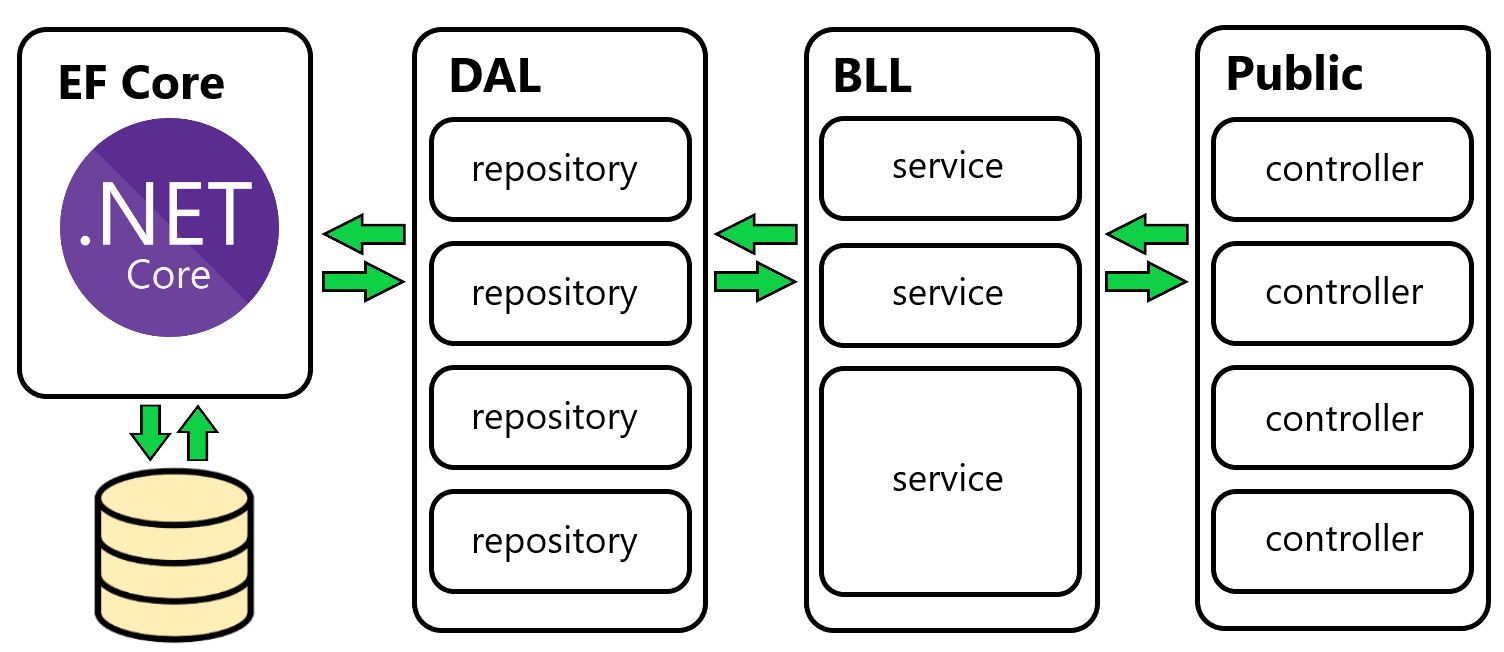
\includegraphics[width=1\textwidth]{figures/development/backend_structure.png}
    \caption[Serveriosa kihtide skemaatiline joonis]{\textit{Serveriosa kihtide skemaatiline joonis}}
    \label{fig:development_backend_layers}
\end{figure}
 

\textbf{EF Core} ja \textbf{Domain} kihis realiseeritakse projekteeritud andmebaasi mudel vastavate klassidena (näiteks \textit{Domain.App.Material},
\textit{Domain.App.Material-Category}, \textit{Domain.App.Material-Property} jne). Igas klassis määratakse olemitele vajalikud omadused ja
olemite vahelised seosed. Domeeni kiht moodustab andmebaasi konteksti (\textit{DbContext}), mis on \textit{Entity Framework Core} raamistiku klass,
mille kaudu raamistik suhtleb andmebaasiga. Raamistiku kaudu luuakse andmebaasi genereerimise ja uuendamise skripte - migratsioonid
(\textit{migration}). Kui üks olemite klassidest oli muudetud, siis uue migratsiooni tegemisel 
võrdleb raamistik uut olekut eelmisega ning genereerib uue skripti.


\textbf{DAL} andmete ligipääsu kihis teostatakse tööd andmebaasi konteksti  objektiga (DbContext):  andmeid küsitakse Entity Framework Core-ist ja 
vastavalt ka salvestatakse \textit{DbContext}-isse. Kiht on jagatud üksusteks -- repositooriumideks (\textit{Repository}), mis on 
baasimplementatsioonis kujutavad ennast klassikalist CRUD-tüüpi repositooriumit. Samuti repositooriumis 
tehakse  andmetele ligipääsu kontrolli kasutaja ID alusel -
nt meetod \textit{GetAllAsync(Guid uid, bool includePublic = false)} vaikimisi küsib andmebaasist kõik olemid, 
mis kuuluvad kasutajale ID-ga \textit{uid} ning valikuliselt lisatakse ka olemeid, mis on ette nähtud ühiskasutuseks. 
\textbf{TODO: Repositooriumi näidiskood, töö Lisa X}

Repositooriumiteks jagamist teostatakse andmemudeli ülesehituse alusel -- iga olemi jaoks on eraldi repositoorium. Selleks, et
äriloogika kihis erinevates teenustes oleks repositooriumite kasutamine paindlik, moodustatakse kõikidest repositooriumitest üks
objekt (\textit{UOW - Unit Of Work} muster), mille kaudu on võimalik juurde pääseda igale repositooriumile.

Kui rakendus vajab mõne olemi puhul keerulisemat repositooriumi loogikat, siis baasfunktsionaalsus saab olla üle kirjutatud
või laiendatud. Näiteks, materjalide (\textit{Domain.App.Material}) puhul on otstarbekam kohe agregeerida andmeid, 
mis puudutavad materjalide omadusi ((\textit{Domain.App.MaterialProperty}) ja (\textit{Domain.App.Property})), siis
äriloogika kihis ei pea tegema lisapäringuid, et teostada vajalikke arvutusi ja tegevusi.


\textbf{BLL} äriloogika kihis toimub andmete põhiline töötlus, mis on seotud vahetult rakenduse funktsionaalsust puudutava loogikaga.
Äriloogika kihi tööüksuseks on teenus (\textit{Service}). Teenuste moodustamise loogika suuresti vastab \textbf{DAL} kihi jagamise loogikale,
et võimalikult isoleerida erinevad teenused omavahelt. On ka teenused, mille eesmärk on erinevatest repositooriumitest andmete agregeerimine --
näiteks, arvutuste teenus (\textit{CalculationService}), mille otstarve on arvutusteks vajalike andmete komplekteerimine kasutajaliidesele
saatmiseks, kasutajaliideselt tulnud arvutuse päringu töötlemine, arvutuste teostamine ja arvutuse tulemuste tagastamine.
\textit{CalculationService} on äriloogika kihi kõike mahukam teenus. Kuna kalkulaatori tööks vajalike andmete maht on suur (materjalide
andmed, konstruktsioonide tüüpidega seotud andmed, sisemiste ja välimiste tingimuste andmed), ei ole otstarbekas
neid kasutajaliidese poolelt küsida eraldi päringutega. Teenuses koostatakse andmete komplekt (\textit{dataset}), mida saadetakse
kasutajaliidesele ühe päringuga.

\textbf{Public} andmete representeerimise kiht tegeleb päringute vastuvõtmisega ja vastuste saatmisega. Kasutajaliideselt päringuga 
tulnud andmed valideeritakse, kontrollides etteantud mudelile vastavust, teisaldatakse äriloogika kihi andmeedastus objektiks
ning antakse üle vastavale äriloogika kihi teenusele. Kuna rakenduse kõigis kihis teatud vea tekkimisel võib programm visata erindeid,
siis tegeleb kiht ka veahaldusega. Vea tekkimisel püütakse seda \textit{try-catch} plokiga kinni ja saadetakse kasutajaliidesele informatiivset
vastus.

Andmebaasiga ühendust haldab raamistik ise. Programmi käivitamise konfiguratsiooni faili (\textit{appsetting.json}) kaudu
antakse raamistikule andmebaasiga ühenduse sõne (\textit{conntection string}), mis sisaldab andmebaasi, kasutajat ja parooli.

Kuna veebirakendus peab kasutama HTTPS protokolli, peab tegema ka vastavad seadistused Asp.NET raamistikus. Asp.NET kasutab päringute
saatmiseks-vastuvõtmisek Kestrel programmi, mis HTTPS protokollil töötamisel vajab serveri SSL sertifikaati. Sertifikaadi
asukoht ja parool antakse raamistikule käivituse konfiguratsiooni failis (\textit{appsetting.json}), millest neid loetakse
ja antake raamistikule programmi käivitamisel failis \textit{Program.cs}: \textbf{koodinäide}.





